\chapter{$t\to qX$ analysis results}
\label{chapter:tqXresults}

In order to test for the presence of a $t\to qX$ signal, a binned maximum-likelihood fit to the data is performed as described in Section~\ref{sec:profilelikelihoodfit}. In total 26 fits are performed, one for each mass hypothesis, fitting in the signal regions the NN output evaluated at the corresponding mass, and the yields in the control regions. The control regions are 4j4b, 5j$\geq$4b and 6j$\geq$4b consist then in one bin, while the three signal regions (4j3b, 5j3b and 6j3b) distributions have ten bins, with irregular binning optimised to increase sensitivity. The parameter of interest is the production of the signal, B($t\to qX$).\\

A total of 282 nuisance parameters are introduced in the fit. To speed up the fit and ease the convergence, the shape or normalisation components of the different systematic uncertainties are pruned if their effect is below a threshold of 0.2\%. In addition, smoothing techniques are applied to reduce the impact of statistical fluctuations when computing the templates of systematic uncertainties.\\

This section provides the expected and observed results on the fitted signal strength, CL$_{\text{s}}$ exclusion limits, a brief review of the $t\to qH$ measurement.

\section{Fit results}

The analysis optimisation is performed on \acrshort{MClabel} simulation and the performance is evaluated via \textit{Asimov} data instead of experimental data. The dataset is built from the nominal background and the chosen signal, thus the normalisation factors and nuisance parameters extracted from the fit are the default ones by construction. Nevertheless, the profile likelihood fit provides uncertainties on the signal strength and the expected upper limits. It is the standard procedure to optimise the analysis without using the experimental data to avoid introducing any bias, especially in signal regions.\\

Once the desired expected sensitivity is obtained and the background modelling reproduces the experimental data in signal-depleted regions, experimental data is added to the fit. Multiple studies were performed to validate the fits studying the effect of pulls and constraints of the nuisance parameters, evaluate possible biases in the signal modelling or evaluating the data/MC agreement in the post-fit distributions among them.\\

Table~\ref{tqX:postfityields} shows the event yields after the $t\to uX$ and $t\to cX$ fits under the 30~GeV X scalar mass fits. Figures~\ref{tqX:NNfit30}, \ref{tqX:NNfit80} and \ref{tqX:NNfit120} show the post-fit distributions of the NN output in the 3b regions and the yields in the $\geq$4b regions for two signal processes and the 30, 80 and 120~GeV $m_X$ hypotheses, respectively. Good agreement between the observed and expected bins is observed after the fit, also seen in the rest of masses and in the input variables of the NN. 

\begin{table}[htb]
    \small
    \centering
    \caption{
    Event yields of the $t\to qX$ signal and background processes in the four analysis regions after the fit to the data under the $X$ scalar mass hypothesis of 30~GeV for $t\to uX$ (top) and $t\to cX$ (bottom).
    The quoted uncertainties take into account correlations and constraints of the nuisance parameters
    and include both the statistical and systematic uncertainties. Negative correlations among \ttb, \ttc\ and \ttl\ modelling uncertainties can cause the uncertainty on the total yields to be smaller than on individual components. \vspace{0.5cm}
    }
    \addtolength{\leftskip} {-2cm} % menja marges
    \addtolength{\rightskip}{-2cm}
    \begin{tabular}{l *{6}{r@{}c@{}l}}
    \toprule\toprule
    \multicolumn{19}{c}{ $t\to uX$, $m_X = 30$~GeV fit}  \\
    \midrule \midrule
    && \makebox[0pt]{4j 3b} &&& \makebox[0pt]{4j 4b} &&& \makebox[0pt]{5j 3b} &&& \makebox[0pt]{5j $\geq$4b} &&& \makebox[0pt]{6j 3b} &&& \makebox[0pt]{6j $\geq$4b}   \\

    \midrule 
    \ttl                & 9300 &$\,\pm\, $&900 & 4.0 &$\,\pm\, $&2.4 & 6200 &$\,\pm\, $&900 & 7 &$\,\pm\, $&5 & 2700 &$\,\pm\, $&500 & 5 &$\,\pm\, $&4 \\ 

    \ttb                  & 11200 &$\,\pm\, $&1000 & 319 &$\,\pm\, $&22 & 15400 &$\,\pm\, $&1200 & 980 &$\,\pm\, $&50 & 12000 &$\,\pm\, $&900 & 1250 &$\,\pm\, $&60 \\ 
    \ttc                    & 3400 &$\,\pm\, $&1100 & 12 &$\,\pm\, $&7 & 4200 &$\,\pm\, $&1300 & 33 &$\,\pm\, $&11 & 2900 &$\,\pm\, $&900 & 29 &$\,\pm\, $&10 \\ 
    $W\rightarrow cb$        & 380 &$\,\pm\, $&60 & 8.1 &$\,\pm\, $&1.2 & 270 &$\,\pm\, $&50 & 11.4 &$\,\pm\, $&1.9 & 132 &$\,\pm\, $&22 & 7.4 &$\,\pm\, $&2.4 \\ 
    Single-$t$              & 1200 &$\,\pm\, $&400 & 19 &$\,\pm\, $&11 & 1100 &$\,\pm\, $&400 & 49 &$\,\pm\, $&22 & 640 &$\,\pm\, $&280 & 60 &$\,\pm\, $&40 \\ 
   $\ttbar H$               & 106 &$\,\pm\, $&14 & 6.6 &$\,\pm\, $&1.0 & 273 &$\,\pm\, $&32 & 45 &$\,\pm\, $&7 & 309 &$\,\pm\, $&35 & 75 &$\,\pm\, $&10 \\ 
    $\ttbar V$               & 120 &$\,\pm\, $&80 & 7 &$\,\pm\, $&5 & 190 &$\,\pm\, $&120 & 25 &$\,\pm\, $&15 & 190 &$\,\pm\, $&120 & 33 &$\,\pm\, $&21 \\ 
    $VV$, $V$+jets        & 870 &$\,\pm\, $&290 & 16 &$\,\pm\, $&5 & 770 &$\,\pm\, $&40 & 28.9 &$\,\pm\, $&3.0 & 459 &$\,\pm\, $&32 & 27.5 &$\,\pm\, $&3.2 \\ 
\midrule  
Signal                   & 10 &$\,\pm\, $&40 & 0.02 &$\,\pm\, $&0.08 & 8 &$\,\pm\, $&33 & 0.2 &$\,\pm\, $&0.8 & 4 &$\,\pm\, $&16 & 0.1 &$\,\pm\, $&0.6 \\
\midrule  
Total                   & 26580 &$\,\pm\, $&170 & 392 &$\,\pm\, $&17 & 28410 &$\,\pm\, $&180 & 1176 &$\,\pm\, $&33 & 19300 &$\,\pm\, $&150 & 1490 &$\,\pm\, $&40 \\  

\midrule
Data                    & & \makebox[0pt]{26614} &&& \makebox[0pt]{374} &&& \makebox[0pt]{28394} &&& \makebox[0pt]{1179} &&& \makebox[0pt]{19302} &&& \makebox[0pt]{1492} \\ 

\bottomrule 
\noalign{\vskip 1cm}  
\toprule
\multicolumn{19}{c}{ $t\to cX$, $m_X = 30$~GeV fit}  \\
\midrule \midrule
&& \makebox[0pt]{4j 3b} &&& \makebox[0pt]{4j 4b} &&& \makebox[0pt]{5j 3b} &&& \makebox[0pt]{5j $\geq$4b} &&& \makebox[0pt]{6j 3b} &&& \makebox[0pt]{6j $\geq$4b}   \\
\midrule 
\ttl    & 10200 &$\,\pm\,$&1200 & 6.4 &$\,\pm\,$&3.3 & 6700 &$\,\pm\,$&1000 & 10 &$\,\pm\,$&6 & 3000 &$\,\pm\,$&600 & 7 &$\,\pm\,$&5 \\ 
\ttb  & 9800 &$\,\pm\,$&1200 & 284 &$\,\pm\,$&25 & 14500 &$\,\pm\,$&1300 & 970 &$\,\pm\,$&50 & 11400 &$\,\pm\,$&1000 & 1250 &$\,\pm\,$&60 \\ 
\ttc   & 3900 &$\,\pm\,$&1300 & 17 &$\,\pm\,$&10 & 4600 &$\,\pm\,$&1400 & 41 &$\,\pm\,$&14 & 3300 &$\,\pm\,$&1100 & 35 &$\,\pm\,$&12 \\ 
$W\rightarrow cb$   & 400 &$\,\pm\,$&60 & 8.7 &$\,\pm\,$&1.2 & 280 &$\,\pm\,$&50 & 12.3 &$\,\pm\,$&2.1 & 134 &$\,\pm\,$&23 & 7.9 &$\,\pm\,$&2.6 \\ 
Single-$t$   & 1200 &$\,\pm\,$&400 & 25 &$\,\pm\,$&15 & 1100 &$\,\pm\,$&400 & 43 &$\,\pm\,$&19 & 550 &$\,\pm\,$&230 & 51 &$\,\pm\,$&31 \\ 
$\ttbar H$   & 109 &$\,\pm\,$&14 & 6.9 &$\,\pm\,$&1.0 & 280 &$\,\pm\,$&33 & 46 &$\,\pm\,$&7 & 316 &$\,\pm\,$&35 & 78 &$\,\pm\,$&11 \\ 
$\ttbar V$   & 140 &$\,\pm\,$&80 & 8 &$\,\pm\,$&5 & 220 &$\,\pm\,$&120 & 28 &$\,\pm\,$&16 & 220 &$\,\pm\,$&120 & 38 &$\,\pm\,$&22 \\ 
$VV$, $V$+jets   & 810 &$\,\pm\,$&260 & 16 &$\,\pm\,$&5 & 730 &$\,\pm\,$&50 & 27.0 &$\,\pm\,$&3.0 & 425 &$\,\pm\,$&34 & 25.0 &$\,\pm\,$&3.0 \\ 
\midrule 
Signal   & 20 &$\,\pm\,$&40 & 0.5 &$\,\pm\,$&1.2 & 14 &$\,\pm\,$&31 & 0.5 &$\,\pm\,$&1.1 & 7 &$\,\pm\,$&15 & 0.4 &$\,\pm\,$&1.0 \\ 
\midrule
Total  & 26600 &$\,\pm\, $&180 & 373 &$\,\pm\, $&18 & 28400 &$\,\pm\, $&190 & 1183 &$\,\pm\, $&34 & 19310 &$\,\pm\, $&150 & 1490 &$\,\pm\,$&40 \\ 
\midrule
Data                    & & \makebox[0pt]{26614} &&& \makebox[0pt]{374} &&& \makebox[0pt]{28394} &&& \makebox[0pt]{1179} &&& \makebox[0pt]{19302} &&& \makebox[0pt]{1492} \\ 
\bottomrule \bottomrule
    \end{tabular}
    \label{tqX:postfityields}
\vspace{1cm}
\end{table}

\begin{figure}[htb]
    \RawFloats
    \centering
    \subfloat[$t\to uX$, 4j3b]{\includegraphics[width = 0.30\textwidth]{TQX/Fits/uX30/c1l4jex3bex_postFit.pdf}}
    \subfloat[$t\to uX$, 5j3b]{\includegraphics[width = 0.30\textwidth]{TQX/Fits/uX30/c1l5jex3bex_postFit.pdf}}
    \subfloat[$t\to uX$, 6j3b]{\includegraphics[width = 0.30\textwidth]{TQX/Fits/uX30/c1l6jex3bex_postFit.pdf}} \\
    \subfloat[$t\to cX$, 4j3b]{\includegraphics[width = 0.30\textwidth]{TQX/Fits/cX30/c1l4jex3bex_postFit.pdf}}
    \subfloat[$t\to cX$, 5j3b]{\includegraphics[width = 0.30\textwidth]{TQX/Fits/cX30/c1l5jex3bex_postFit.pdf}}  
    \subfloat[$t\to cX$, 6j3b]{\includegraphics[width = 0.30\textwidth]{TQX/Fits/cX30/c1l6jex3bex_postFit.pdf}} \\ 
    \subfloat[$t\to uX$, $\geq$4b]{\includegraphics[width = 0.30\textwidth]{TQX/Fits/uX30/Summary_postFit.pdf}} 
    \subfloat[$t\to cX$, $\geq$4b]{\includegraphics[width = 0.30\textwidth]{TQX/Fits/cX30/Summary_postFit.pdf}}    
    \caption{Comparison between the data and prediction for the NN output in the 3b regions for the $t\to uX$ ((a) to (c))
    and the $t\to cX$\ ((d) to (f)) processes, 
    and the yields in the $\geq$4b regions for the $t\to uX$ (g) and the $t\to cX$ (h) processes 
    after the signal-plus-background fit to data for corresponding fit under the 30 GeV $X$ scalar mass hypothesis.}
    \label{tqX:NNfit30}
\end{figure}

\begin{figure}[htb]
    \RawFloats
    \centering
    \subfloat[$t\to uX$, 4j3b]{\includegraphics[width = 0.30\textwidth]{TQX/Fits/uX80/c1l4jex3bex_postFit.pdf}}
    \subfloat[$t\to uX$, 5j3b]{\includegraphics[width = 0.30\textwidth]{TQX/Fits/uX80/c1l5jex3bex_postFit.pdf}}
    \subfloat[$t\to uX$, 6j3b]{\includegraphics[width = 0.30\textwidth]{TQX/Fits/uX80/c1l6jex3bex_postFit.pdf}} \\
    \subfloat[$t\to cX$, 4j3b]{\includegraphics[width = 0.30\textwidth]{TQX/Fits/cX80/c1l4jex3bex_postFit.pdf}}
    \subfloat[$t\to cX$, 5j3b]{\includegraphics[width = 0.30\textwidth]{TQX/Fits/cX80/c1l5jex3bex_postFit.pdf}}  
    \subfloat[$t\to cX$, 6j3b]{\includegraphics[width = 0.30\textwidth]{TQX/Fits/cX80/c1l6jex3bex_postFit.pdf}} \\ 
    \subfloat[$t\to uX$, $\geq$4b]{\includegraphics[width = 0.30\textwidth]{TQX/Fits/uX80/Summary_postFit.pdf}} 
    \subfloat[$t\to cX$, $\geq$4b]{\includegraphics[width = 0.30\textwidth]{TQX/Fits/cX80/Summary_postFit.pdf}}    
    \caption{Comparison between the data and prediction for the NN output in the 3b regions for the $t\to uX$ ((a) to (c))
    and the $t\to cX$\ ((d) to (f)) processes, 
    and the yields in the $\geq$4b regions for the $t\to uX$ (g) and the $t\to cX$ (h) processes 
    after the signal-plus-background fit to data for the corresponding fit under the 80 GeV $X$ scalar mass hypothesis.}
    \label{tqX:NNfit80}
\end{figure}

\begin{figure}[htb]
    \RawFloats
    \centering
    \subfloat[$t\to uX$, 4j3b]{\includegraphics[width = 0.30\textwidth]{TQX/Fits/uX120/c1l4jex3bex_postFit.pdf}}
    \subfloat[$t\to uX$, 5j3b]{\includegraphics[width = 0.30\textwidth]{TQX/Fits/uX120/c1l5jex3bex_postFit.pdf}}
    \subfloat[$t\to uX$, 6j3b]{\includegraphics[width = 0.30\textwidth]{TQX/Fits/uX120/c1l6jex3bex_postFit.pdf}} \\
    \subfloat[$t\to cX$, 4j3b]{\includegraphics[width = 0.30\textwidth]{TQX/Fits/cX120/c1l4jex3bex_postFit.pdf}}
    \subfloat[$t\to cX$, 5j3b]{\includegraphics[width = 0.30\textwidth]{TQX/Fits/cX120/c1l5jex3bex_postFit.pdf}}  
    \subfloat[$t\to cX$, 6j3b]{\includegraphics[width = 0.30\textwidth]{TQX/Fits/cX120/c1l6jex3bex_postFit.pdf}} \\ 
    \subfloat[$t\to uX$, $\geq$4b]{\includegraphics[width = 0.30\textwidth]{TQX/Fits/uX120/Summary_postFit.pdf}} 
    \subfloat[$t\to cX$, $\geq$4b]{\includegraphics[width = 0.30\textwidth]{TQX/Fits/cX120/Summary_postFit.pdf}}    
    \caption{Comparison between the data and prediction for the NN output in the 3b regions for the $t\to uX$ ((a) to (c))
    and the $t\to cX$\ ((d) to (f)) processes, 
    and the yields in the $\geq$4b regions for the $t\to uX$ (g) and the $t\to cX$ (h) processes 
    after the signal-plus-background fit to data for the corresponding fit under the 120 GeV $X$ scalar mass hypothesis.}
    \label{tqX:NNfit120}
\end{figure}


\clearpage

The nuisance parameters and normalisation factors are different to the original values, as the fit accommodates for normalisation and shape differences between the observed and predicted distributions.\\

The signal strength and the \ttb\ and \ttc\ normalisation nuisance parameters are summarised in Figure~\ref{tqX:fittedfactorsvsmass}. The \ttb\ normalisation nuisance parameter ranges from 0.19 to 0.56 (0.10 to 0.49) with a typical uncertainty of 0.25 (0.24) for the $t\to uX$ ($t\to cX$) fits, while the \ttc\ parameter ranges from 0.29 to 1.10 (-0.13 to 1.02) with a typical uncertainty of 0.79 (0.47). Regarding the signal strength, the largest deviations with respect to the \acrshort{SMlabel} hypothesis are observed for $m_X=80$~GeV  and $m_X=40$~GeV hypotheses for the $t\to cX$ and $t\to uX$, respectively. $t\to uX$ shows some negative deviations which does not represent evidence of the signal.\\

Figure~\ref{tqX:p0values} shows the $p_0$ values corresponding to the significance as a function of $m_X$ and for both types of signal. The $t\to cX$ process shows larger but constant $\sim$2$\sigma$ deviations in the 40--120~GeV range which peaks at $m_X=80$~GeV with 2.2$\sigma$, while the $t\to uX$ has a more defined peak at 40~GeV equivalent to 1.8$\sigma$. The difference between the $t\to uX$ and $t\to cX$ results is not only from the difference in statistics, they slightly differ in the fourth jet due to its different flavour. Given the use of $b$-tagging information in the NN training, the discrimination achieved between background and $t\to uX$ or $t\to cX$ signals slightly differs too and depends on the mass of the scalar.\\

\begin{figure}[htb]
    \RawFloats
    \centering
    \subfloat[$t\to uX$]{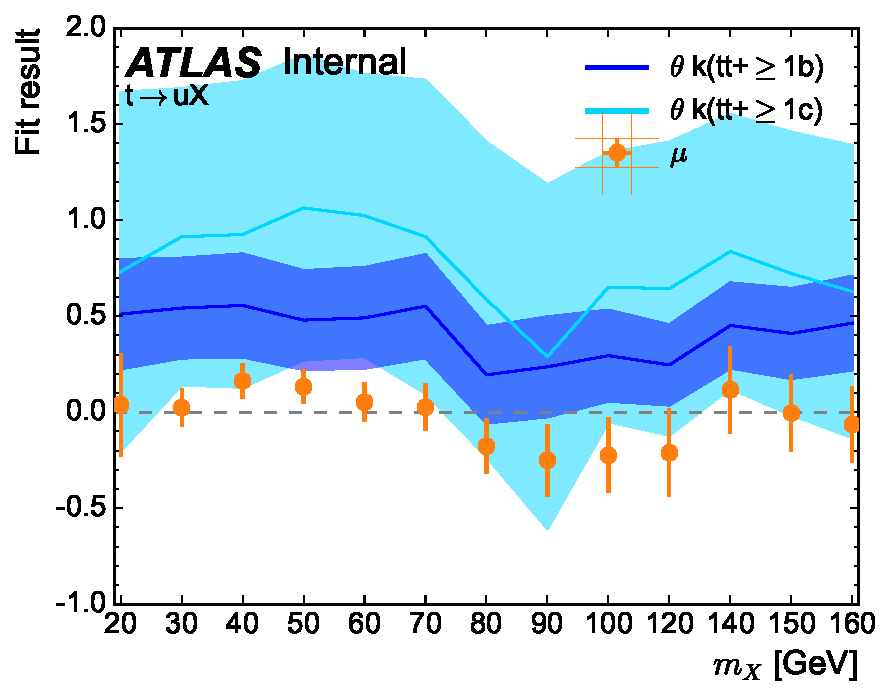
\includegraphics[width = 0.45\textwidth]{TQX/Fits/Fitvsmass_sbv10cRWv3_u.pdf}}
    \subfloat[$t\to cX$]{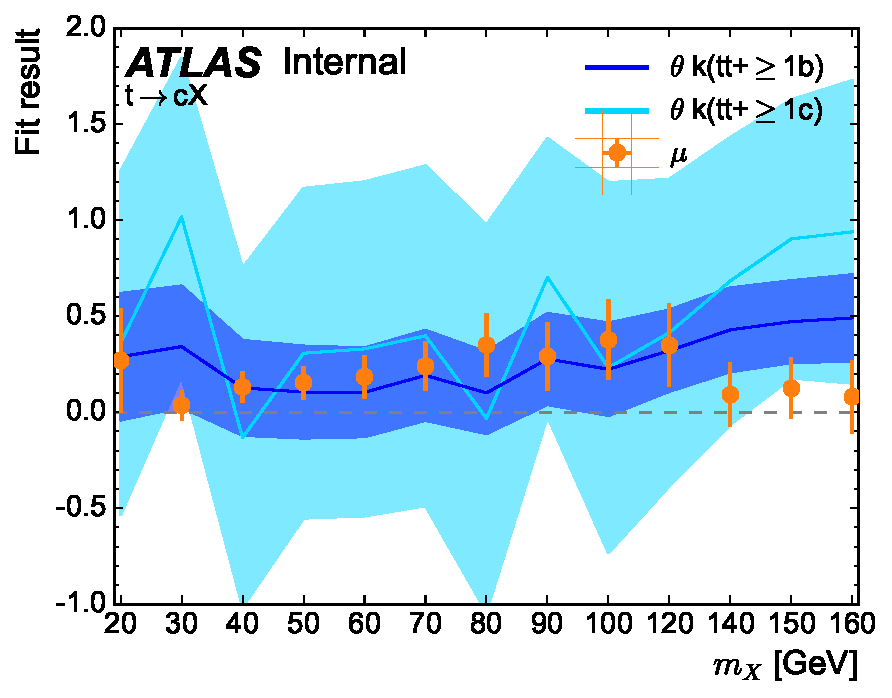
\includegraphics[width = 0.45\textwidth]{TQX/Fits/Fitvsmass_sbv10cRWv3_c.pdf}}
    \caption{Evolution of the obtained signal strength and the nuisance parameters related to the \ttb\ and \ttc\ normalisation as a function of the $X$ scalar mass with the corresponding uncertainties. The signal strength is normalised to 0.1\% branching fraction.
    }
    \label{tqX:fittedfactorsvsmass}
\end{figure}

\begin{figure}[htb]
    \RawFloats
    \centering
    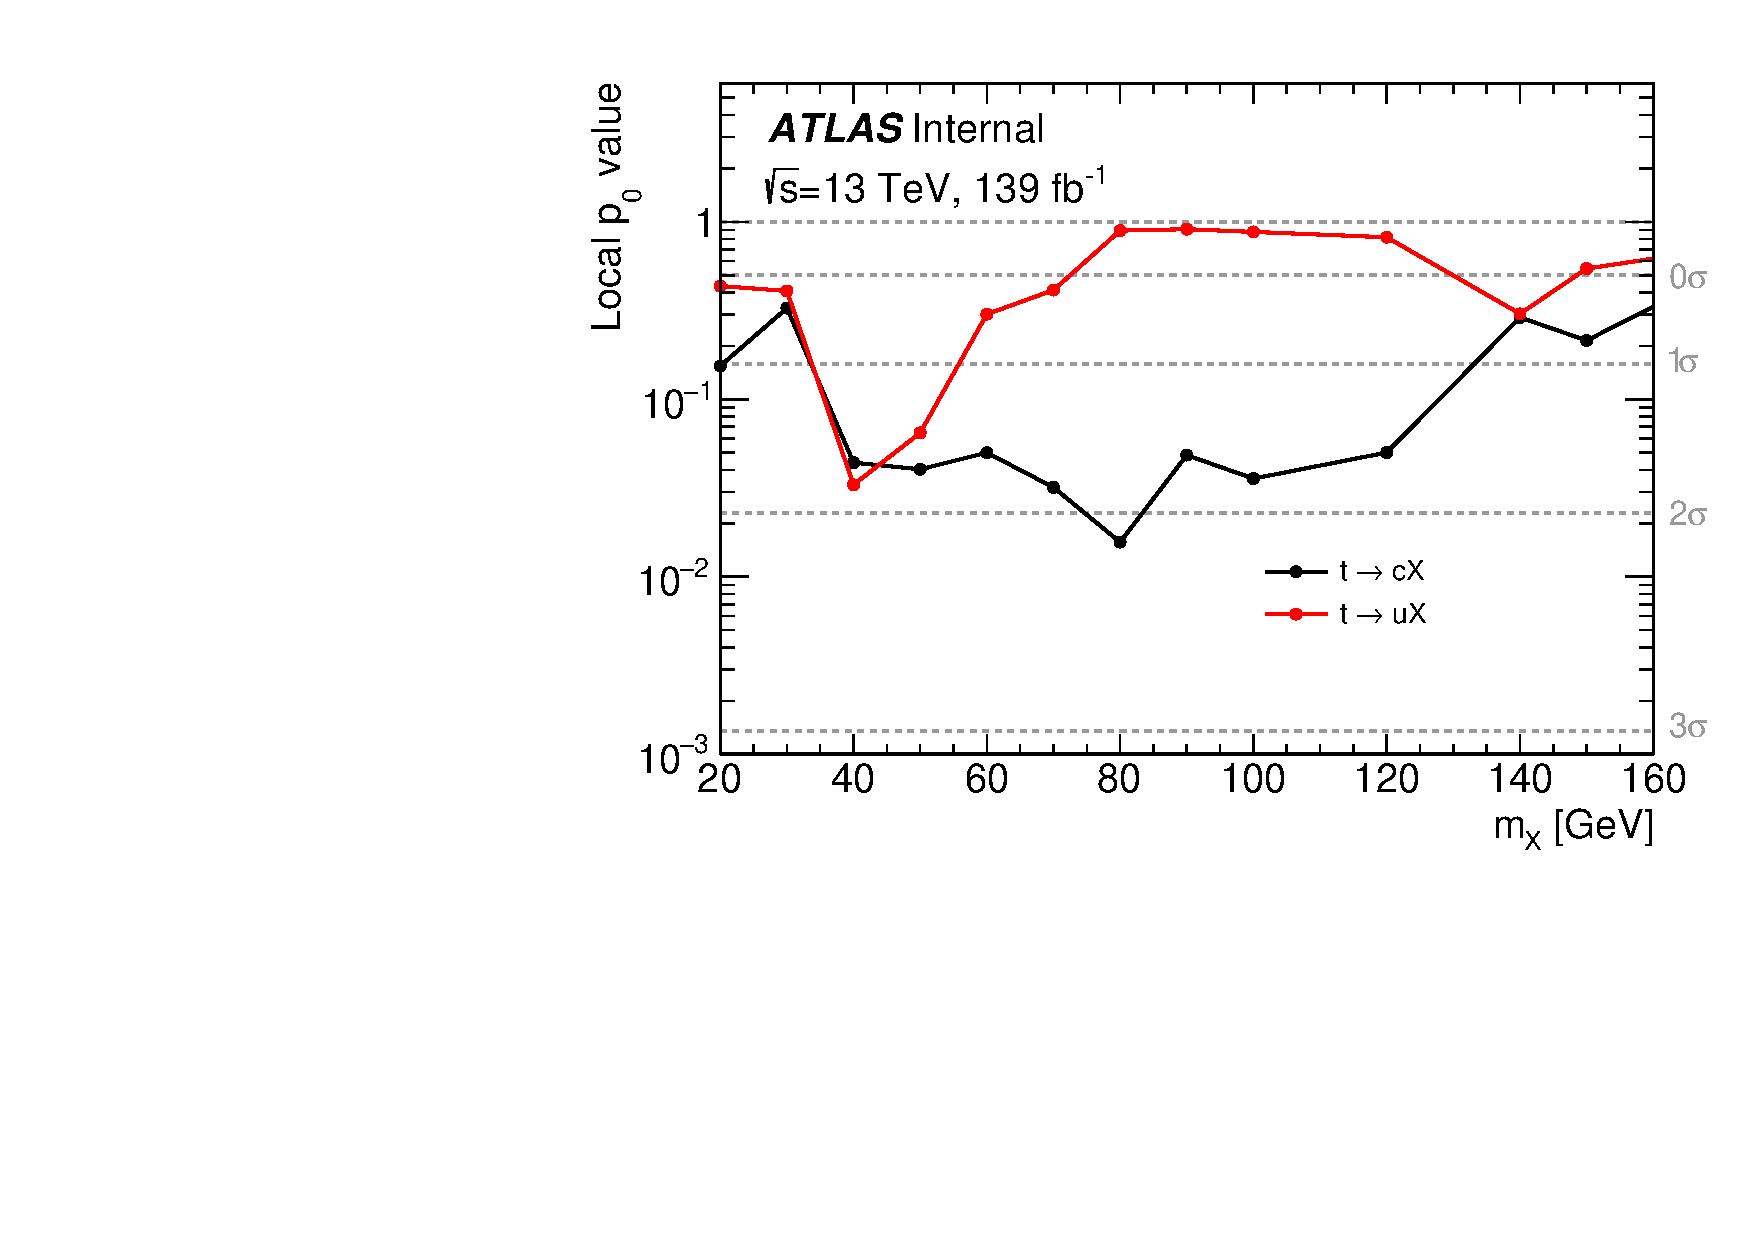
\includegraphics[width =0.49\textwidth]{TQX/Fits/pzero_v10cRW_v2.pdf}
    \caption{$p_0$ values for the fitted signal strength as a function of the mass of $X$ hypothesis for the $t\to cX$ (black) and $t\to uX$ (red) signal fits.}
    \label{tqX:p0values}
\end{figure}
\clearpage
\subsection{Dominant uncertainties}

The uncertainty associated to the fit result is mainly driven by systematic uncertainties. The different sources are ranked by the impact on the signal strength in terms of its shift from the default result $\Delta\mu$, evaluated in separate fits where the associated nuisance parameters are fixed to $\hat{\theta}\pm\Delta\hat{\theta}$. $\hat{\theta}$ is the best fit value of the given nuisance parameter while $\Delta\hat{\theta}$ is the corresponding one standard deviation.\\

Figure~\ref{tqX:ranking3080120} lists the 20 top ranked nuisance parameters of the 30, 80 and 120~GeV $m_X$ hypothesis fits for both types of signal. The upper axis represents the scale for the pre-fit and post-fit impact on $\mu$. The pre-fit (post-fit) impact is given as $\hat{\theta} \pm \Delta\theta (\hat{\theta} \pm \Delta\hat{\theta})$, with $\Delta\theta$ ($\Delta\hat{\theta}$) the pre-fit (post-fit) uncertainties. The post-fit value of $\Delta\hat{\theta}$ is typically smaller than the one standard deviation prior, $\Delta\theta$, due to constraints from the fit to data. The pre-fit and post-fit impacts are shown as empty and filled rectangles, respectively. The lower axis indicates the scale of the pull of the nuisance parameter defined as $\frac{\hat{\theta} -\theta_0}{\Delta\theta}$ with $\theta_0$ the nominal pre-fit value. The pulls are indicated as black points with their respective error bar while the single-bin statistical uncertainties ($\gamma$) are drawn with $\theta_0=0$ and without the pre-fit impact, as it is not properly defined.\\

\begin{figure}[htb]
    \RawFloats
    \addtolength{\leftskip} {-2cm} % menja marges
    \addtolength{\rightskip}{-2cm}
    \centering
    \subfloat[$t\to uX$, $m_X = 30$~GeV]{\includegraphics[width = 0.45\textwidth]{TQX/Fits/uX30/Ranking_mu_XS.pdf}}
    \subfloat[$t\to cX$, $m_X = 30$~GeV]{\includegraphics[width = 0.45\textwidth]{TQX/Fits/cX30/Ranking_mu_XS.pdf}}\\
    \subfloat[$t\to uX$, $m_X = 80$~GeV]{\includegraphics[width = 0.45\textwidth]{TQX/Fits/uX80/Ranking_mu_XS.pdf}}
    \subfloat[$t\to cX$, $m_X = 80$~GeV]{\includegraphics[width = 0.45\textwidth]{TQX/Fits/cX80/Ranking_mu_XS.pdf}}\\
    \subfloat[$t\to uX$, $m_X = 120$~GeV]{\includegraphics[width = 0.45\textwidth]{TQX/Fits/uX120/Ranking_mu_XS.pdf}}
    \subfloat[$t\to cX$, $m_X = 120$~GeV]{\includegraphics[width = 0.45\textwidth]{TQX/Fits/cX120/Ranking_mu_XS.pdf}}
    %\subfloat[$t\to uX$, $m_X = 30$~GeV]{\includegraphics[width = 0.45\textwidth]{TQX/Fits/uX30/Ranking_mu_XS.pdf}}
    %\subfloat[$t\to uX$, $m_X = 80$~GeV]{\includegraphics[width = 0.45\textwidth]{TQX/Fits/uX80/Ranking_mu_XS.pdf}}
    %\subfloat[$t\to uX$, $m_X = 120$~GeV]{\includegraphics[width = 0.45\textwidth]{TQX/Fits/uX120/Ranking_mu_XS.pdf}}\\
    %\subfloat[$t\to cX$, $m_X = 30$~GeV]{\includegraphics[width = 0.45\textwidth]{TQX/Fits/cX30/Ranking_mu_XS.pdf}}
    %\subfloat[$t\to cX$, $m_X = 80$~GeV]{\includegraphics[width = 0.45\textwidth]{TQX/Fits/cX80/Ranking_mu_XS.pdf}}
    %\subfloat[$t\to cX$, $m_X = 120$~GeV]{\includegraphics[width = 0.45\textwidth]{TQX/Fits/cX120/Ranking_mu_XS.pdf}}\\
    \caption{Ranking of the 20 systematic uncertainties with the largest impact on $\mu$ for the fit performed with the 30~GeV (a, d), 80~GeV (b, e), 120~GeV (c, f) $m_X$ hypothesis and both $t\to qX$ processes. The empty (filled) rectangles correspond  to the pre-fit (post-fit) impact on $\mu$. The black points represent the post-fit pulls of the nuisance parameters relative to the nominal values, $\theta_0$. Statistical uncertainties ($\gamma$) are shown pulled with respect to 1.
    }
    \label{tqX:ranking3080120}
\end{figure}

The five highest-ranked nuisance parameters of the presented $t\to uX$ signal hypothesis fit include the 4j component of the different \ttjets\ PS or \ttl\ NLO matching, the \ttc\ normalisation, the statistical component of the last bin of the 4j3b distributions or a component of the $c$-tagging efficiency. Regarding the $t\to cX$ fits, the five highest-ranked across masses include the \ttb\ and \ttc\ normalisations, components of the light- and $c$-tagging, 4j component of \ttb\ PS/NLO and \ttl\ PS, 5j component of \ttb\ 5FS vs 4FS and the statistics of the mentioned bin.\\

Table~\ref{tqX:rankingbreakuX} and Table~\ref{tqX:rankingbreakcX} shows, for both $t\to qX$ processes, the impact on the signal strength evaluated in groups of systematic uncertainty sources for the 30, 80 and 120~GeV signal hypothesis fits. The total uncertainty is dominated by the systematic uncertainties, where \ttb\ modelling dominates for all masses except $t\to uX$ at $m_X=120$, where one of the $b$-tagging components dominates. In general, the \ttb\ modelling dominates, followed by the modelling of the other two components or those from $b$-tagging.\\

\clearpage
\begin{table}[htb]
    \caption{
      Summary of the statistical and systematic uncertainties on $\mu=\text{B}(t\to uX)$ for the 30, 80 and 120~GeV $X$ scalar mass hypothesis fits. Due to correlations between the different sources of uncertainty, the total systematic uncertainty can be different from the sum in quadrature of the individual sources.}
    \begin{center}
    \begin{tabular}{l c c c}
    \toprule\toprule
    Uncertainty source   & $\Delta\mu(uX_{30})$ & $\Delta\mu(uX_{80})$ & $\Delta\mu(uX_{120})$ \\
    \midrule \midrule
    \ttb\ modelling	                       &	0.040	&	0.060	&	0.098	\\
    \ttc\ modelling	                       &	0.033	&	0.055	&	0.091	\\
    \ttl\ modelling         	           &	0.034	&	0.058	&	0.040	\\
    \ttb\ normalisation                  	   &	0.012	&	0.011	&	0.039	\\
    \ttc\ normalisation	                   &	0.017	&	0.036	&	0.087	\\  
    $W\rightarrow cb$ modelling	               &	0.001	&	0.010   &	0.017	\\
    Reweighting	                               &	0.005	&	0.013	&	0.017	\\
    Other backgrounds                          &	0.008	&	0.026	&	0.023	\\
    Luminosity, JVT, pile-up            	   &	0.002	&	0.006	&   0.012 	\\
    Lepton trigger, identification, isolation  &	0.001	&	0.004	&	0.007	\\
    Jet energy scale and resolution	           &	0.008	&	0.037	&	0.040	\\
    $b$-tagging efficiency for $b$-jets  	   &	0.007	&	0.008	&	0.041	\\
    $b$-tagging efficiency for $c$-jets        &	0.014	&	0.027	&	0.079	\\
    $b$-tagging efficiency for light jets      &	0.007	&	0.008	&	0.010	\\
    \MET	                                   &	0.002	&	0.010	&	0.011	\\
    \midrule
    Total systematic uncertainty        	   &	0.077	&	0.125	&	0.220	\\
    \midrule
    Signal statistical uncertainty	           &	0.014	&	0.009	&	0.007	\\
    \midrule
    Total statistical uncertainty	           &	0.064	&	0.070	&	0.065	\\
    \midrule \midrule
    Total uncertainty           	           &	0.098	&	0.141	&	0.230	\\
    \bottomrule \bottomrule
  \end{tabular}
  \end{center}
  \label{tqX:rankingbreakuX}
  \end{table}

  \begin{table}[htb]
    \caption{
      Summary of the statistical and systematic uncertainties on $\mu=\text{B}(t\to cX)$ for the 30, 80 and 120~GeV $X$ scalar mass hypothesis fits. Due to correlations between the different sources of uncertainty, the total systematic uncertainty can be different from the sum in quadrature of the individual sources.}
    \begin{center}
    \begin{tabular}{l c c c}
    \toprule\toprule
    Uncertainty source   & $\Delta\mu(cX_{30})$ & $\Delta\mu(cX_{80})$ & $\Delta\mu(cX_{120})$ \\
    \midrule \midrule
    \ttb\ modelling	                       &	  0.034	&	0.074	&	0.079	\\
    \ttc\ modelling	                       &	  0.010	&	0.012	&	0.040	\\
    \ttl\ modelling	                       &	  0.008	&	0.049	&	0.038	\\
    \ttb\ normalisation       	           &	  0.026	&	0.038	&	0.001	\\
    \ttc\ normalisation	                   &	  0.019	&	0.048	&	0.013	\\
    $W \rightarrow cb$ modelling               &	0.001	&	0.020	&	0.015	\\
    Reweighting	                               &  	0.005	&	0.013	&	0.019	\\
    Other backgrounds            	           &	0.009	&	0.057	&	0.047	\\
    Luminosity, JVT, pile-up	               &	0.005	&	0.005	&	0.003	\\
    Lepton trigger, identification, isolation  &	0.001	&	0.004 	&	0.003  \\
    Jet energy scale and resolution	           &	0.017	&	0.049	&	0.051	\\
    $b$-tagging efficiency for $b$-jets        &	0.003	&	0.016	&	0.023	\\
    $b$-tagging efficiency for $c$-jets	       &	0.010	&	0.038	&	0.091	\\
    $b$-tagging efficiency for light jets      &	0.009	&	0.065	&	0.125	\\
    \MET	                                   &	0.001	&	0.003	&	0.008	\\
    \midrule
    Total systematic uncertainty	           &	0.056	&	0.150	&	0.208	\\
    \midrule
    Signal statistical uncertainty             &	0.017	&	0.012	&	0.008	\\
    \midrule
    Total statistical uncertainty	           &	0.064	&	0.067	&	0.058	\\
    \midrule \midrule
    Total uncertainty	                       &	0.079	&	0.162	&	0.217	\\
    \bottomrule \bottomrule
  \end{tabular}
  \end{center}
  \label{tqX:rankingbreakcX}
  \end{table}
  
\clearpage

\section{Exclusion limits}

No significant excess above the expected \acrshort{MClabel} background is observed in all regions and mass intervals, hence upper limits on the signal production are derived as function of the $X$ scalar mass.\\

Figure~\ref{tqX:xseclimits} shows the 95\% confidence level (CL) upper limits on B($t\to uX$)$\times$B($X\to\bbar$) and B($t\to uX$)$\times$B($X\to\bbar$), obtained using the CL$_\text{S}$ method. An excess of 1.8$\sigma$ is seen in the $t\to uX$ channel at $m_X=40$~GeV. Also, a roughly two-standard deviation excess can be seen in the $t\to cX$ observed limit over almost the entire range of $m_X$. As mentioned before, this excess is not compatible with the presence of a scalar particle $X$, which would show up as a narrower, resonance-like, excess in the limit plot.\\

The observed (expected) limits range from 0.019\% (0.017\%) to 0.062\% (0.056\%) for B($t\to uX$)$\times$B($X\to\bbar$) and from 0.018\% (0.015\%) to 0.078\% (0.056\%) for B($t\to cX$)$\times$B($X\to\bbar$).\\

\begin{figure}[htb]
    \RawFloats
    \centering
    \subfloat[$t\to uX$]{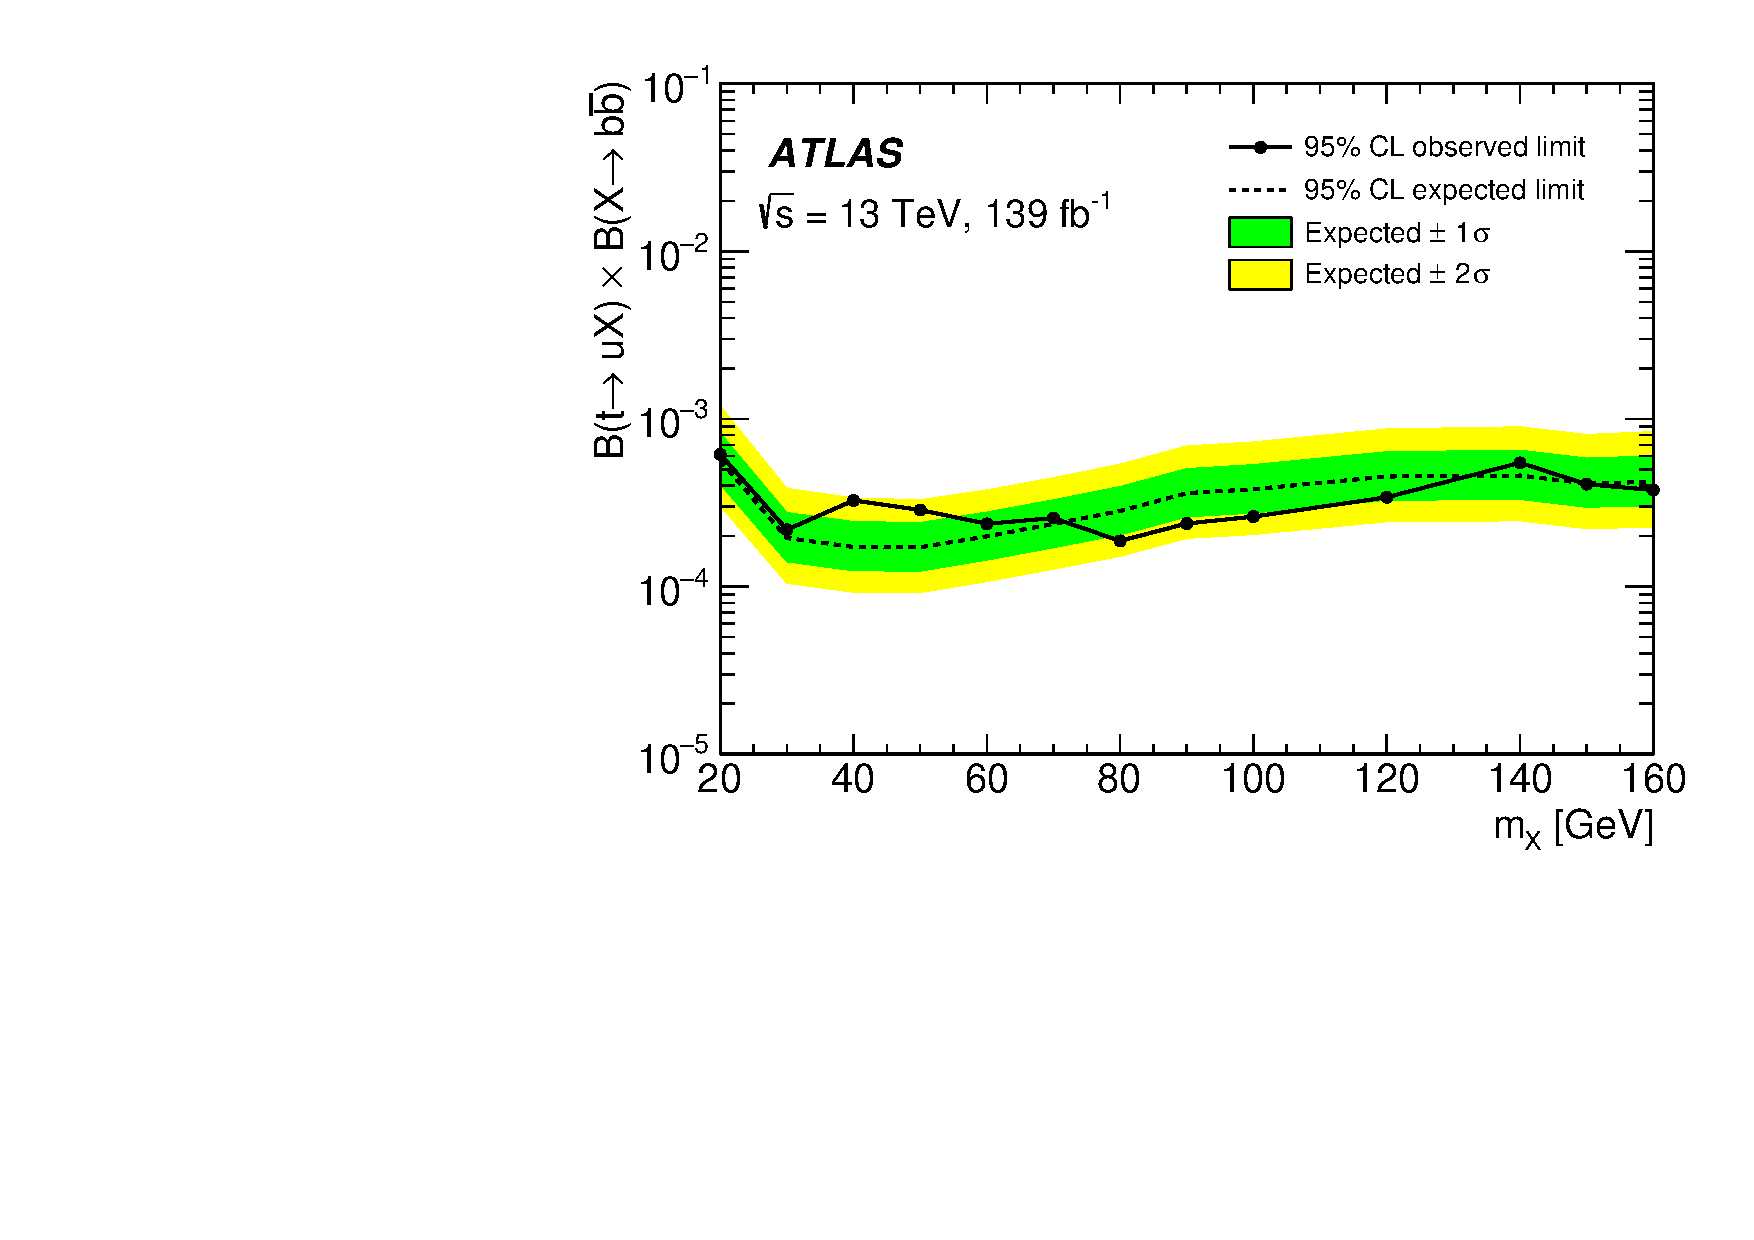
\includegraphics[width = 0.6\textwidth]{TQX/Fits/Limit_BR_v10cRW_v2_u_noint.pdf}}\\
    \subfloat[$t\to uX$]{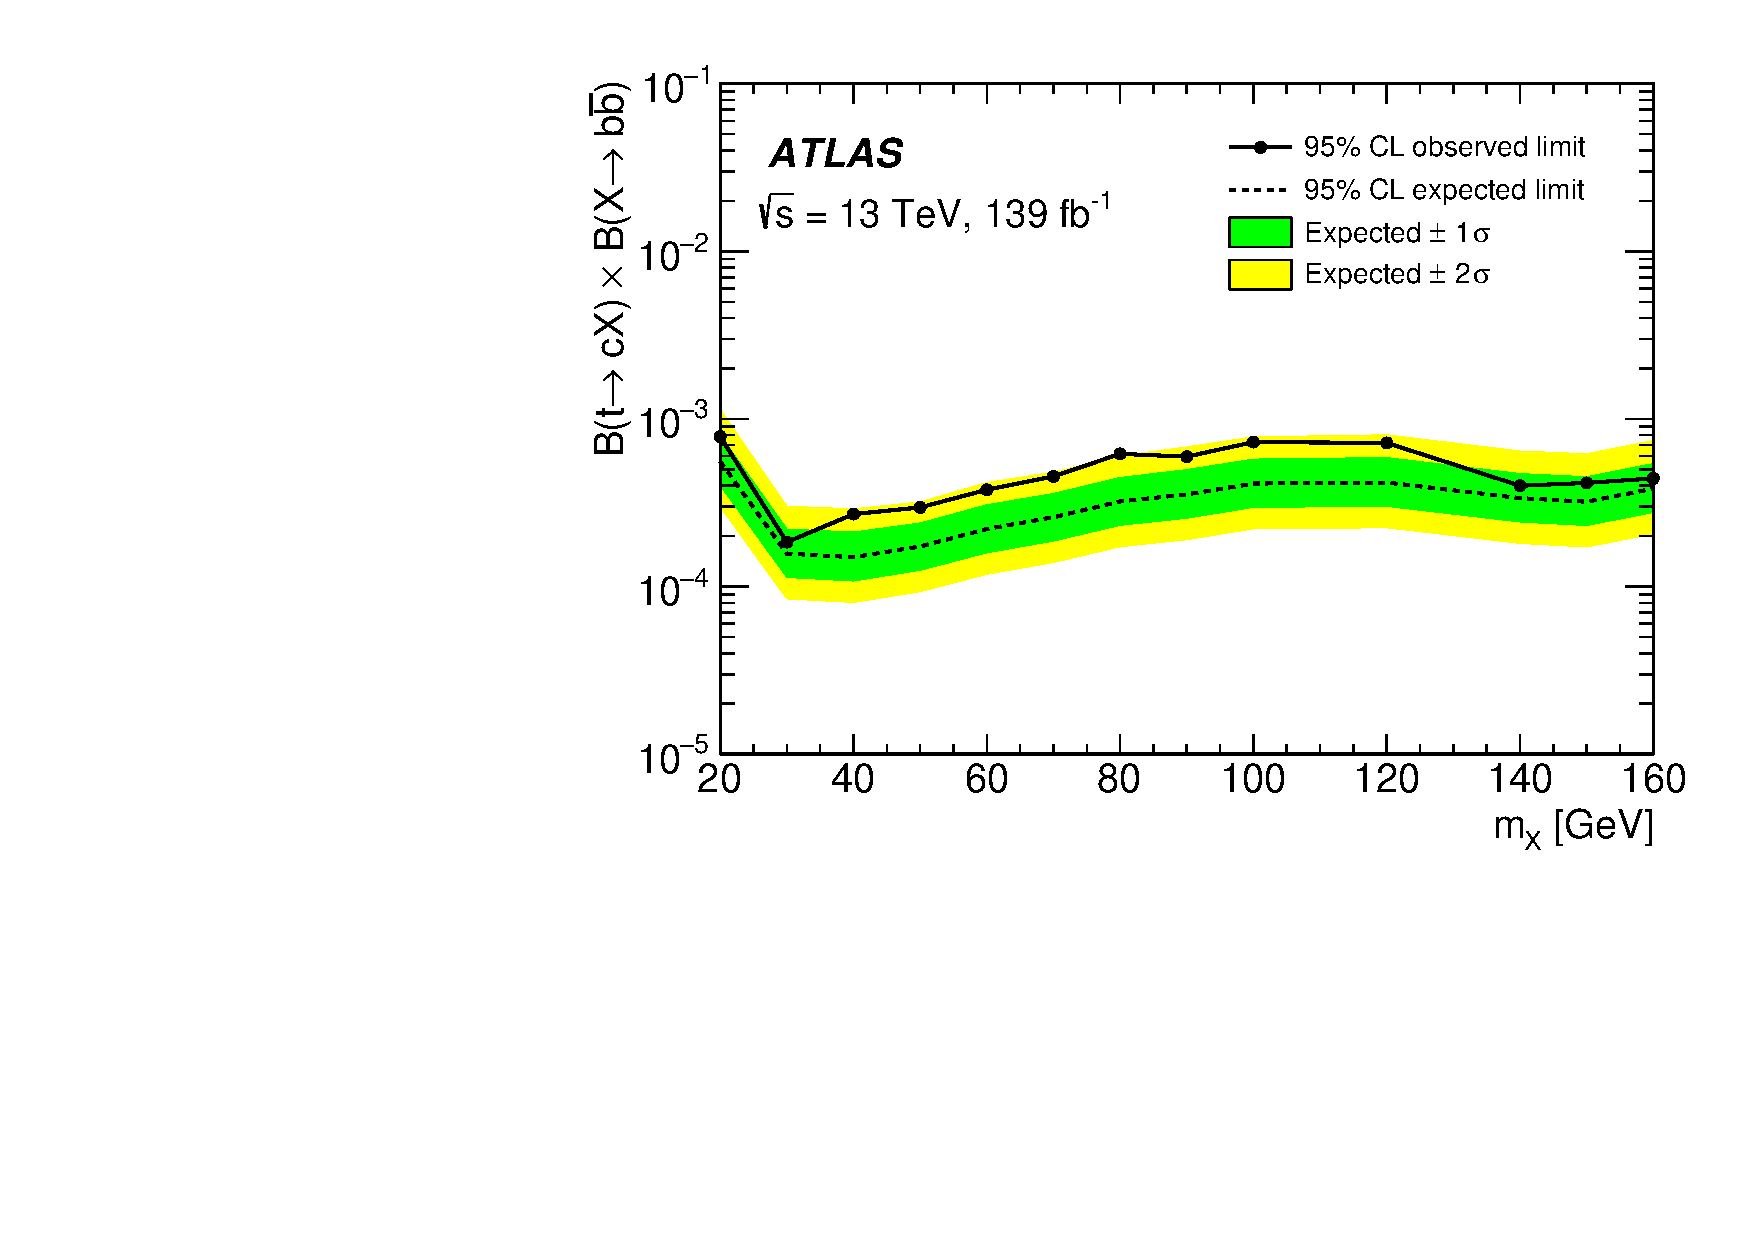
\includegraphics[width = 0.6\textwidth]{TQX/Fits/Limit_BR_v10cRW_v2_c_noint.pdf}}
    \caption{Observed and expected upper limits for B($t\to uX$)$\times$B($X\to\bbar$) (a) and B($t\to uX$)$\times$B($X\to\bbar$) (b) as a function of the $X$ scalar mass. The bands surrounding the expected limit show the 68\% and 95\% confidence intervals.}
    \label{tqX:xseclimits}
\end{figure}

\section{$t\to qH$ measurement}

Two additional fits are performed for the $t\to uH$ and $t\to cH$ processes, involving the \acrshort{SMlabel} Higgs boson. The samples are simulated with the same generators as the rest of the signal samples: the \ttbar\ pair is produced using the \POWHEGBOX v2 generator interfaced to \MADSPIN and \PYTHIA~8.2, with one of the tops decaying leptonically and the second one decaying to a charm or an up quark together with the Higgs boson. The Higgs is left to decay according to the \acrshort{SMlabel} branching ratios. Similarly, no sample of single top production in association with the Higgs boson has been included.\\

Thanks to the use of a parameterised NN, its evaluation using a mass hypothesis different from any of the signal samples used in the training is possible. The NN output scores for the $t\to uH$ and $t\to cH$ signal samples as well as the different background samples are evaluated using the mass hypothesis corresponding to the Higgs mass, $m_H=125$~GeV. The performance of the NN is close to the evaluation at $m_X=120$, and has to be close to ideal as the $m_H=125$~GeV value is not far from the mass used in the training.\\

Two fits corresponding to the $t\to uH$ and $t\to cH$ hypotheses have been performed using the same method, regions and background modelling as for the rest of the hypotheses. The fitted $\mu$ is $-0.19\pm0.44$ for $t\to uH$ and $0.51\pm0.39$ for $t\to uH$. Figure~\ref{tqX:RankqH} shows the top ranked nuisance parameter for both the $t\to uH$ and $t\to cH$ fits. As expected, no big differences in pulls are observed when compared with the fits corresponding to the 120~GeV scalar mass hypothesis (Figure~\ref{tqX:ranking3080120}).\\

\begin{figure}[htb]
    \RawFloats
    \centering
    \subfloat[$t\to uH$]{\includegraphics[width = 0.45\textwidth]{TQX/Fits/Higgs/uH/Ranking_mu_XS.pdf}}
    \subfloat[$t\to cH$]{\includegraphics[width = 0.45\textwidth]{TQX/Fits/Higgs/cH/Ranking_mu_XS.pdf}}
    \caption{Ranking of the 20 systematic uncertainties with the largest impact on $\mu$ for the fit performed with the \acrshort{SMlabel} Higgs hypothesis and both $t\to qH$ processes. The empty (filled) rectangles correspond  to the pre-fit (post-fit) impact on $\mu$. The black points represent the post-fit pulls of the nuisance parameters relative to the nominal values, $\theta_0$. Statistical uncertainties ($\gamma$) are shown pulled with respect 1.}
    \label{tqX:RankqH}
\end{figure}

Branching ratio upper limits for both $t\to uH$ and $t\to cH$ hypotheses have been extracted. The observed (expected) upper limits are $7.6\times10^{-4}$ ($11.8\times10^{-4}$) and $8.8\times10^{-4}$ ($7.7\times10^{-4}$) for B($t\to uH$) and B($t\to cH$), respectively. Figure~\ref{tqX:limitIncH} shows the upper limits for the $t\to uH$ and $t\to cH$ hypotheses including the fit results with the 125~GeV mass, which, only for illustrating the compatibility with the rest of the mass fits, have been scaled assuming a B(H$\rightarrow b \bar{b}) = 100\%$ instead of the \acrshort{SMlabel} branching ratio of 58\%. A very good compatibility with a poor-man extrapolation from the 120 to 140~GeV mass fit results can be observed.\\

\begin{figure}[htb]
    \RawFloats
    \centering
    \subfloat[$t\to uX$]{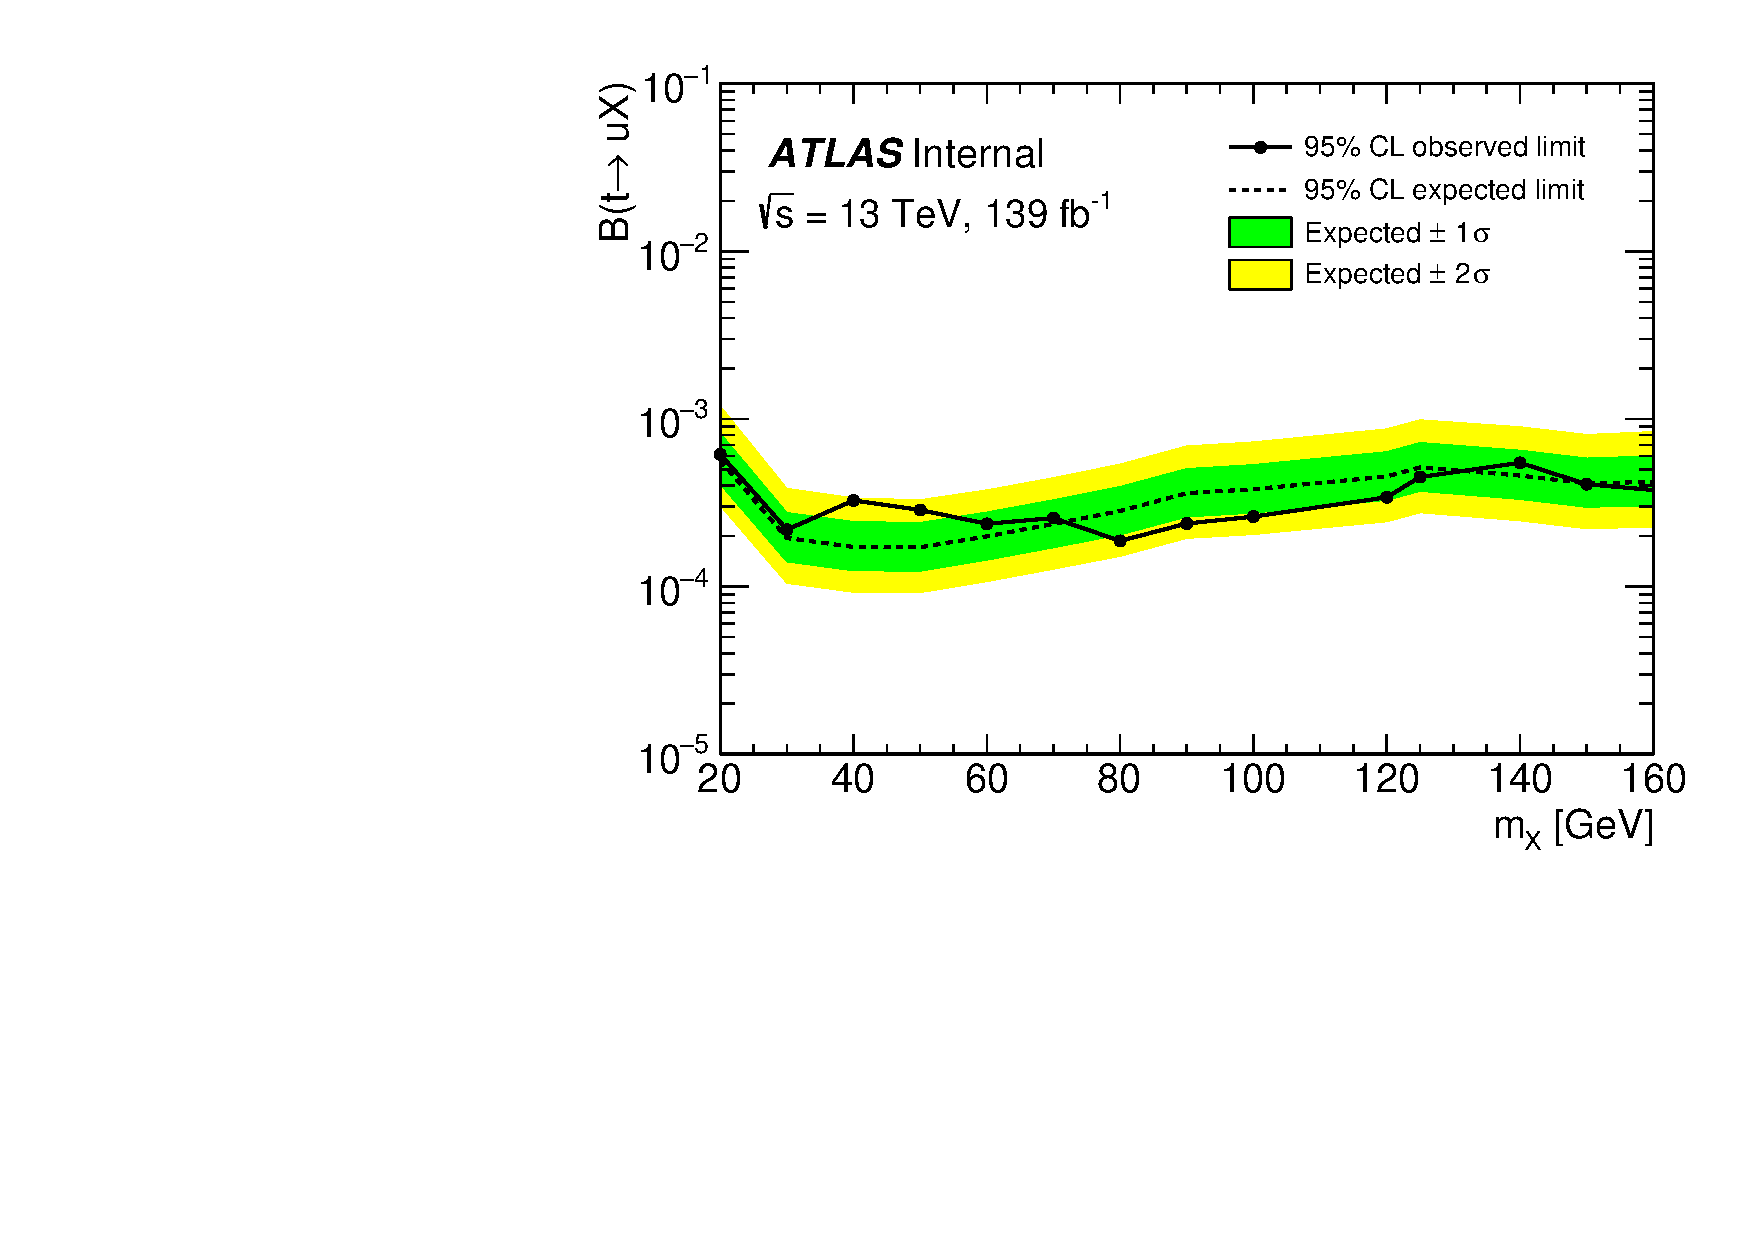
\includegraphics[width =0.495\textwidth]{TQX/Fits/Higgs/Limit_BR_v10cRW_125e_u.pdf}}
    \subfloat[$t\to uX$]{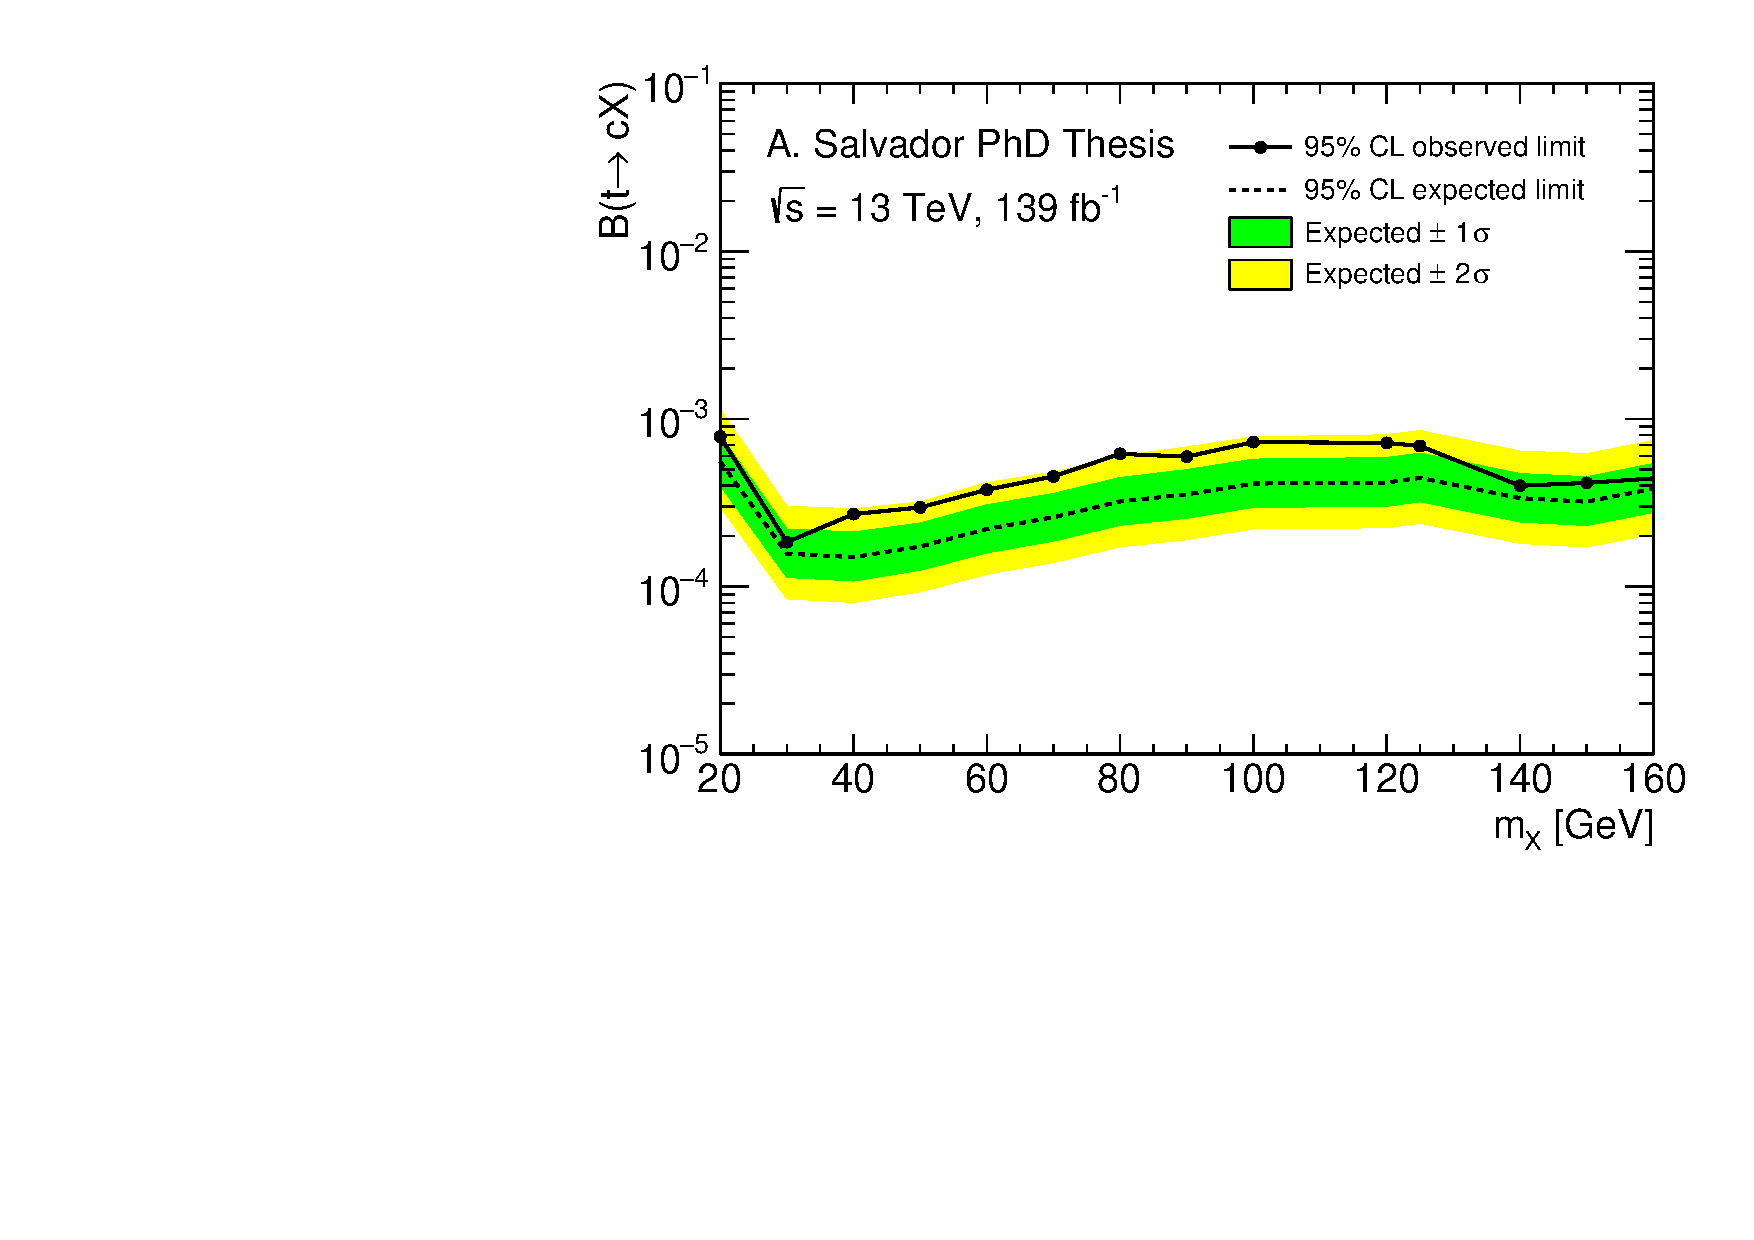
\includegraphics[width =0.495\textwidth]{TQX/Fits/Higgs/Limit_BR_v10cRW_125e_c.pdf}}
    \caption{Observed and expected upper limits for B($t\to uX$)$\times$B($X\to\bbar$) (a) and B($t\to cX$)$\times$B($X\to\bbar$) (b) as a function of the $X$ scalar mass. The bands surrounding the expected limit show the 68\% and 95\% confidence intervals. The upper limits corresponding to the Higgs boson mass hypothesis have been scaled down assuming B($H \rightarrow b \bar{b}) = 100\%$.}
    \label{tqX:limitIncH}
\end{figure}

Figure~\ref{tqX:cHlimitcomparison} shows a comparison of different upper limits results: the result of $t\to cX$ for the 120~GeV hypothesis, the $t\to cH$ result presented in this section, the CMS $t\to cH$ result with 137~fb$^{-1}$ data~\cite{CMStqHRun2}, and the $t\to cH$ ATLAS result with 36~fb$^{-1}$ data~\cite{TOPQ-2017-07}. It should be noted that the $t\to cX$ upper limit assumes a B(X$\rightarrow b \bar{b}$) = 100\%, while 58\% is assumed for the \acrshort{SMlabel} Higgs decay.\\

Previously published results by \acrshort{ATLASlabel} and CMS include the single-top signal sample in the analyses while, as mentioned above, this sample is not included in this analysis. The comparison is only presented for the decay involving the $c$-quark as the effect of including the single-top process is negligible. It can be observed that the expected limits obtained are on average a factor of three better than the previous \acrshort{ATLASlabel}, scaled to the same integrated luminosity, and slightly better than the CMS results.

\begin{figure}[htb]
    \RawFloats
    \centering
    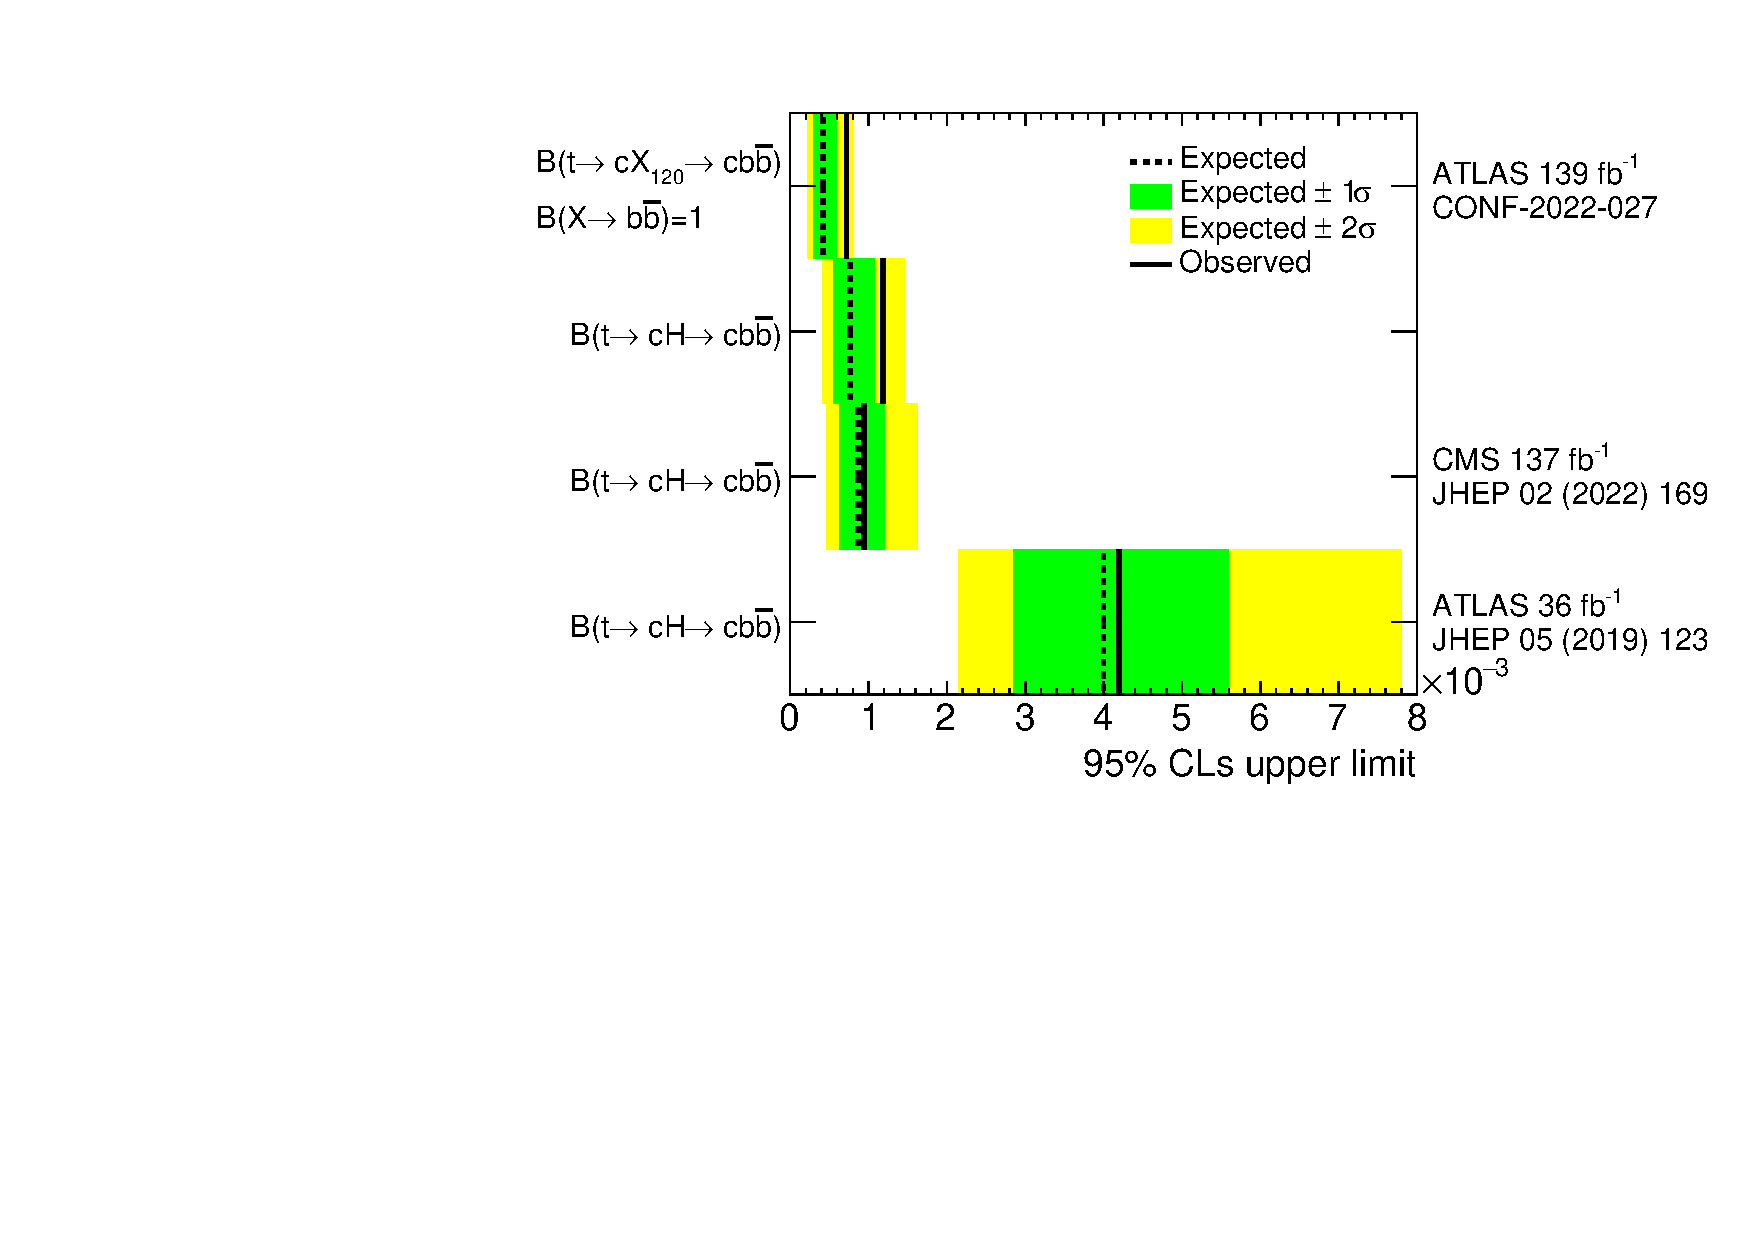
\includegraphics[width =0.7\textwidth]{TQX/Fits/Higgs/tcXcomparison.pdf}
    \caption{Expected and observed upper limits for the branching ratio of different $t\to cX$ results. The results shown include the $t\to cX$ results for the 120~GeV mass hypothesis, the $t\to cX$ result presented in this section and the $t\to cX$ published results from FCNC searches performed by CMS using 137~fb$^{-1}$ and by ATLAS using 36~fb$^{-1}$. The bands surrounding the expected limits show the 68\% and 95\% confidence intervals.}
    \label{tqX:cHlimitcomparison}
\end{figure}


% \section{Outlook}

% first trial, lots of refining

% lower correlations
% optimise NN for the different regimes, for individual regions or combining tcX and tuX (ended up promoting tcX training). Low level information is very useful, complement with more high level variables
% Tried to include an extra step of a NN trained only with signal to reconstruct the resonance, was being used as high level input for the classification NN, with minor improvements not bein able to justify the effor. Tried GNN to see if more info can be extracted
% Tried parameterising the NN to be able to evaluate for different key systematics
% Use kinematical discriminant like past iterations of tqH. (And used in H+tb)

% lower correlations
% CEvent categorisation, btagging important so maybe custom stronger btagging or splitting further in different PCBT would enhance the signal, although we are at the edge of statistics ucnertainties for some bins

%include single-top and lower jet regions.